\chapter{Categories of Shots}
\label{ch:categories}

Chapter~\ref{ch:editing} met the category $\Path(\Sc)$ in passing. This chapter develops the categorical vocabulary needed to speak about film, namely categories, functors, and monoidal structure, and uses it to give a precise account of the relation between a world and its images and of the simultaneous composition of picture and sound. Appendix~\ref{app:cat} collects the definitions; the reader meeting the subject for the first time should read it alongside this chapter.

\section{Categories, functors, and the rendering functor}

A \emph{category} $\mathbf{C}$ consists of objects, morphisms between them, an associative composition, and identities. A \emph{functor} $F:\mathbf{C}\to\mathbf{D}$ assigns objects to objects and morphisms to morphisms so as to preserve composition and identities~\cite{maclane1998}.

\begin{proposition}[Rendering as a functor]\label{prop:rendering-functor}
Let $(\Sc,\Ren)$ be a scenario space. Then $\Ren$ induces a functor $\Ren_*:\Path(\Sc)\to\Path(\Img)$ with $\Ren_*(s)=\Ren(s)$ on objects and $\Ren_*(\tau,\gamma)=(\tau,\Ren\circ\gamma)$ on morphisms.
\end{proposition}

\begin{proof}
Since $\Ren$ is continuous, $\Ren\circ\gamma$ is a Moore path in $\Img$ from $\Ren(\gamma(0))$ to $\Ren(\gamma(\tau))$. Composition and identities are preserved because post-composition with $\Ren$ commutes with concatenation of paths and takes constant paths to constant paths.
\end{proof}

The proposition says that what the audience sees of a seamless take is determined by what happens in the world, in a way that respects the joining of takes. When $\Ren$ has positive-dimensional fibers, $\Ren_*$ fails to be faithful, which is the technical statement that different takes can look identical: two distinct morphisms of $\Path(\Sc)$ may have the same image. (Non-injectivity alone does not force this: a covering map is non-injective, yet paths lift uniquely.) It typically fails to be full as well, because most image paths do not arise from continuous paths of world states, which is the formal content of the idea that cinema can show what no physical set could produce.

\begin{example}[Faithful but not essentially surjective]
Suppose $\Ren$ is an embedding. Then $\Ren_*$ is faithful, because $\Ren\circ\gamma=\Ren\circ\gamma'$ implies $\gamma=\gamma'$, and the image of $\Ren_*$ consists of paths in $\Img$ that lie in $\Ren(\Sc)$. If $\Ren(\Sc)$ is a proper subset of $\Img$, which is generic, then $\Ren_*$ is not essentially surjective. A dissolve between two shots produces an image path leaving $\Ren(\Sc)$, so it is not in the image of any functor of this form; it must be modeled by a separate operation on $\Path(\Img)$ and not by a movement of the world.
\end{example}

\section{Products and the synchronization of tracks}

A film is more than a picture. Sound, picture, and subtitles run in parallel and are required to be synchronized. Categorically this is a limit construction.

Consider two scenario spaces $\Sc_1$ and $\Sc_2$, for instance the visual world and the acoustic world. Moore paths in the product $\Sc_1\times\Sc_2$ are pairs of Moore paths of the same duration.

\begin{proposition}[Synchronization as a fiber product]\label{prop:fiber}
The category $\Path(\Sc_1\times\Sc_2)$ is isomorphic to the fiber product of categories
\[
\Path(\Sc_1)\times_{(\R_{\ge0},+)}\Path(\Sc_2),
\]
taken over the two duration functors. Explicitly, its objects are pairs $(s_1,s_2)$ and its morphisms are pairs of morphisms with equal duration.
\end{proposition}

\begin{proof}
A Moore path $(\tau,(\gamma_1,\gamma_2))$ in the product has components that are Moore paths of the same duration $\tau$, and conversely any pair of Moore paths of equal duration assembles into a path in the product. Composition and identities are computed componentwise, with durations adding in both components simultaneously. The map is bijective on objects and morphisms and preserves composition, hence is an isomorphism of categories.
\end{proof}

This is the mathematical form of the editor's rule that picture and sound may be cut at different places but must sum to the same running time. A film in which the sound track is allowed to lead or lag the picture, as in the L-cut and J-cut, is not a path in the product but a pair of paths whose seams are offset, and this offset is exactly the failure of the pair to be composed of morphisms of the fiber product at each seam. The relaxed structure, in which durations are required to agree only in total, is the subject of Exercise~\ref{ex:lcut}.

\section{Monoidal structure and string diagrams}

The fiber product is a special case of monoidal composition. A \emph{monoidal category} has, in addition to composition of morphisms in sequence, a tensor product that composes them in parallel, subject to coherence conditions. Pictures called \emph{string diagrams} represent such compositions: sequential composition runs downward, parallel composition runs across~\cite{selinger2011}.

\begin{figure}[ht]
\centering
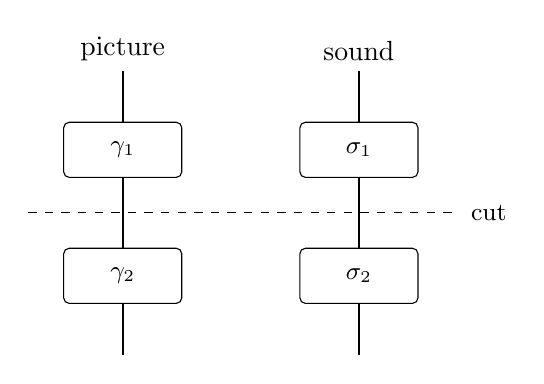
\begin{tikzpicture}[
  box/.style={draw, rounded corners=2pt, minimum width=1.5cm, minimum height=0.7cm, font=\small},
  wire/.style={thick}
]
\node[box] (p1) at (0,0)   {$\gamma_1$};
\node[box] (s1) at (3,0)   {$\sigma_1$};
\node[box] (p2) at (0,-1.6){$\gamma_2$};
\node[box] (s2) at (3,-1.6){$\sigma_2$};
\draw[wire] (0,1) node[above]{picture} -- (p1);
\draw[wire] (p1) -- (p2);
\draw[wire] (p2) -- (0,-2.6);
\draw[wire] (3,1) node[above]{sound} -- (s1);
\draw[wire] (s1) -- (s2);
\draw[wire] (s2) -- (3,-2.6);
\draw[dashed] (-1.2,-0.8) -- (4.2,-0.8);
\node[right] at (4.3,-0.8) {\small cut};
\end{tikzpicture}
\caption{A two-track film as a string diagram. Vertical composition is the sequence of shots on each track, and horizontal juxtaposition is parallel composition. A synchronized cut crosses both strands at the same level.}
\label{fig:string}
\end{figure}

What the monoidal viewpoint adds is a way of stating when tracks are independent. Two edits on different tracks are independent when the film's change is a tensor $g\otimes g'$ of a change $g$ on one track and a change $g'$ on the other. Composition then satisfies the interchange law
\[
(g\circ f)\otimes(g'\circ f')=(g\otimes g')\circ(f\otimes f').
\]
When this holds, it does not matter whether one thinks of the film as first doing both first-shots and then both second-shots, or as doing each track's two shots in turn. The interchange law itself is an axiom of every monoidal category, so it cannot fail. What can fail is that a given edit is of the form $g\otimes g'$. A sound effect whose meaning depends on the exact image it overlays is a change of the pair that is not a tensor of changes on the tracks, and this is a coupling between them. (In a premonoidal category, where only one track can advance at a time, interchange itself may fail; we do not need that refinement.)

\section{Kuleshov, revisited}

The superadditive interpretation $\mu$ of Chapter~\ref{ch:editing} keeps its form: it is a lax monoidal functor from the word monoid $\Sigma^*$, with concatenation as tensor, to a monoidal preorder of meanings, with comparison $\mu(u)\otimes\mu(v)\le\mu(uv)$ going from parts to whole. A lax monoidal functor need not be strong, and the cases in which it is not are the cases that film theory calls montage. Whether a comparable structure exists on $\Path(\Sc)$ depends on choosing a monoidal structure there, which we do not do; the claim of this section concerns concatenation of shots.

\section{Bridge: three kinds of composition}

Three different operations are all called composition in editing, and the forged-letter scene exhibits each. \emph{Composing tracks} places dialogue over a picture. This is the fiber product of \Cref{prop:fiber}: the two tracks have equal duration and run in parallel, and nothing is added to the running time. \emph{Composing events} places one event after another in the history. Consider a reaction shot of $B$ inserted at $t=62$. If the shot is inserted into the timeline as a new segment of four seconds, the monoid homomorphism $\dur$ adds four seconds and every later event is delayed. If the same four seconds of picture replace the picture under existing dialogue, the sound track continues unchanged and the running time is the same. Insertion and overlay are different operations, with different effects on $\dur$, and a film description that does not say which was used does not determine the running time. \emph{Composing an interpretation} concerns what the reaction shot does to the meaning of the reveal that precedes it. This is the lax structure of the previous sections, and it is not an operation on picture or sound at all.

The rendering functor $\Ren_*$ preserves the first two by definition: it preserves the joining of takes and the durations of paths. It does not preserve the third. Music that continues across a cut, which is widely understood to smooth the perceived transition, is a relation between the sound track and the seam in the picture, and neither the scenario path nor the rendering contains it as a morphism. Likewise the inference that $B$ is shaken by the reveal is not a morphism in $\Path(\Img)$. Whatever relates a seam to its perceived continuity or a shot to its expressive meaning must be supplied by an interpretation functor into a category of meanings, and, as argued above, such a functor is in general only lax.

\section*{Exercises}

\begin{exercise}
Show that the duration map $\dur:\Path(\Sc)\to(\R_{\ge0},+)$ is a functor and that it is faithful if and only if for each pair of points $s,s'$ there is at most one Moore path of each duration from $s$ to $s'$. Under what conditions on $\Sc$ does this fail?
\end{exercise}

\begin{exercise}\label{ex:lcut}
Define a category of two-track films in which the durations of the two tracks need agree only in total, and describe its relation to the fiber product of \Cref{prop:fiber}. Which edits are morphisms of the fiber product and which require the larger category?
\end{exercise}

\begin{exercise}
In the setting of \Cref{prop:rendering-functor}, let $\Ren':\Sc\to\Img$ be a second rendering with $\Ren'=\Ren$ on a subspace $\Sc_0\subset\Sc$. Show that $\Ren_*$ and $\Ren'_*$ agree on the full subcategory $\Path(\Sc_0)$.
\end{exercise}
